\documentclass[twocolumn]{article}
% do not change these values
\baselineskip 12pt
\textheight 9in
\textwidth 6.5in
\oddsidemargin 0in
\topmargin 0in
\headheight 0in
\headsep 0in

%\documentclass{sig-alternate}
\setlength{\pdfpagewidth}{8.5truein}
\setlength{\pdfpageheight}{11truein}

\usepackage{times}
\usepackage{epsfig}
\usepackage{amsmath}
\usepackage{amsfonts}
\usepackage[tight]{subfigure}
%\usepackage{cite}
\usepackage{url}
\usepackage{mathptmx}
%\usepackage[usenames,dvipsnames]{color}
\usepackage[export]{adjustbox}
\usepackage[justification=centering]{caption}

\widowpenalty=100000
\clubpenalty=100000



\usepackage{upgreek}

\newcommand{\fixme}[1]{{\Large FIXME:} {\bf #1}}
\newcommand{\XXX}[1]{{\Large XXX:} {\it #1}}
%\newcommand{\MYnote}[1]{{\Large Note:} {\bf #1}}
%\newcommand{\MYcomment}[1]{ {\Large Comment:} {\bf #1}}
\newcommand{\MYcomment}[1]{}
\renewcommand{\figurename}{Fig.}
\newcommand{\us}{$\upmu$s~}
\newcommand{\MYnote}[1]{}
\newcommand{\MYgt}{\textgreater}
\newcommand{\MYlt}{\textless}
\newcommand{\MYu}[1]{\underline{#1}}

\newcommand{\MYequationref}[1]{Equation~\ref{#1}}
\newcommand{\MYsectionref}[1]{Section~\ref{#1}}
\newcommand{\MYsectionsref}[2]{Sections~\ref{#1}~and~\ref{#2}}
\newcommand{\MYfigureref}[1]{Figure~\ref{#1}}
\newcommand{\MYalgorithmref}[1]{Algorithm~\ref{#1}}
\newcommand{\MYfiguresref}[2]{Figures~\ref{#1}~and~\ref{#2}}
\newcommand{\MYtableref}[1]{Table~\ref{#1}}
\newcommand{\MYsmall}{\small}
\newcommand{\MYtablefontsize}{\small}
\newcommand{\MYcaptionfontsize}{\small }

\newcommand{\MYetal}{\textit{et~al.}}
\newcommand{\MYie}{{\em i.e.}}
\newcommand{\MYeg}{{\em e.g.}}
\newcommand{\MYetc}{{\em etc.}}

\newcommand{\MYfootnote}[2]{{\footnote[#1]{#2} }}
\newcommand{\MYparagraph}[1]{{\vspace{0.1in} \noindent \bf #1: }}

\newcounter{MYtablecntr}
\addtocounter{MYtablecntr}{1}
\newcommand{\MYtablepicf}[3]{{
  \renewcommand{\thefigure}{\arabic{MYtablecntr}}
  \renewcommand{\figurename}{Tab.}
    \begin{figure*}
      \centering
      \includegraphics[scale=1.0]{#2}%[scale=0.9]
    \caption{#3}
    \label{#1}
   \end{figure*}
  \addtocounter{MYtablecntr}{1}
}}

\newcommand{\MYtablepich}[3]{{
  \renewcommand{\thefigure}{\arabic{MYtablecntr}}
  \renewcommand{\figurename}{Tab.}
    \begin{figure}[h!]
      \centering
      \includegraphics[scale=0.95]{#2}%[scale=0.9]
    \caption{#3}
    \label{#1}
   \end{figure}
  \addtocounter{MYtablecntr}{1}
}}

\newcommand{\MYtablepic}[3]{{
  \renewcommand{\thefigure}{\arabic{MYtablecntr}}
  \renewcommand{\figurename}{Tab.}
    \begin{figure}
      \centering
      \includegraphics[scale=1.0]{#2}%[scale=0.9]
    \caption{#3}
    \label{#1}
   \end{figure}
  \addtocounter{MYtablecntr}{1}
}}

\newcounter{MYalgorithmcntr}
\addtocounter{MYalgorithmcntr}{1}
\newcommand{\MYalgorithmpic}[3]{{
  \renewcommand{\thefigure}{\arabic{MYalgorithmcntr}}
  \renewcommand{\figurename}{Alg.}
    \begin{figure}[t]
      \centering
      \includegraphics[scale=1.0]{#2}%[scale=0.9]
    \caption{#3}
    \label{#1}
   \end{figure}
  \addtocounter{MYalgorithmcntr}{1}
}}


\newenvironment{MYitemize}{\begin{list}{}{%
\setlength{\topsep}{3pt plus 0pt minus 0pt}%
\setlength{\itemsep}{5pt plus 0pt minus 0pt}%
\setlength{\parsep}{1pt plus 0pt minus 0pt}%
\setlength{\parskip}{1pt plus 0pt minus 0pt}%
\setlength{\leftmargin}{15pt}%
}}{\end{list}}

\newenvironment{MYwideitemize}{\begin{list}{}{%
\setlength{\topsep}{3pt plus 0pt minus 0pt}%
\setlength{\itemsep}{5pt plus 0pt minus 0pt}%
\setlength{\parsep}{1pt plus 0pt minus 0pt}%
\setlength{\parskip}{0pt plus 0pt minus 0pt}%
\setlength{\parindent}{0pt }
\setlength{\leftmargin}{0pt}%
}}{\end{list}}

\newcommand{\MYlabel}{\small {$\bullet$}}
\newenvironment{MYlist}{\begin{list}{\MYlabel}{%
\setlength{\topsep}{3pt plus 0pt minus 0pt}%
\setlength{\itemsep}{5pt plus 0pt minus 0pt}%
\setlength{\parsep}{1pt plus 0pt minus 0pt}%
\setlength{\parskip}{1pt plus 0pt minus 0pt}%
}}{\end{list}}

\newenvironment{MYlistwide}{\begin{list}{\MYlabel}{%
\setlength{\topsep}{2pt plus 0pt minus 0pt}%
\setlength{\itemsep}{2pt plus 0pt minus 0pt}%
\setlength{\parsep}{2pt plus 0pt minus 0pt}%
\setlength{\parskip}{0pt plus 0pt minus 0pt}%
\setlength{\parindent}{0pt }
\setlength{\leftmargin}{0pt}%
}}{\end{list}}

\newcounter{MYenumctrtwo}
\newenvironment{MYenumwide}{\begin{list}{\arabic{MYenumctrtwo}.}{%
\usecounter{MYenumctrtwo}%
\setlength{\topsep}{2pt plus 0pt minus 0pt}%
\setlength{\itemsep}{2pt plus 0pt minus 0pt}%
\setlength{\parsep}{2pt plus 0pt minus 0pt}%
\setlength{\parskip}{0pt plus 0pt minus 0pt}%
\setlength{\parindent}{0pt }
\setlength{\leftmargin}{15pt}%
}}{\end{list}}


\newcounter{MYenumctr}
\newenvironment{MYenum}{\begin{list}{\arabic{MYenumctr}.}{%
\usecounter{MYenumctr}%
\setlength{\topsep}{3pt plus 0pt minus 0pt}%
\setlength{\itemsep}{5pt plus 0pt minus 0pt}%
\setlength{\parsep}{1pt plus 0pt minus 0pt}%
\setlength{\parskip}{1pt plus 0pt minus 0pt}%
}}{\end{list}}


\newcommand{\naive}{na\"\i{}ve}
\newcommand{\Naive}{Na\"\i{}ve}

\newcommand{\JK}{\textcolor{green}}

\newcommand{\LC}[1]{{\color{blue} #1}}
 \newcommand{\LYC}[1]{{\color{red} Lydia: #1}}
\newcommand{\zlScale}{$40M$~}

%set dimensions of columns, gap between columns, and space between paragraphs
\setlength{\textheight}{9.0in}
\setlength{\textwidth}{6.5in}
%\setlength{\columnsep}{0.15in}
%\setlength{\footskip}{0.0in}
%\setlength{\topmargin}{0.0in}
%\setlength{\headheight}{0.0in}
%\setlength{\headsep}{0.0in}
%\setlength{\oddsidemargin}{0.0in}
%\setlength{\evensidemargin}{0.0in}
%\setlength{\parindent}{0pc}
%%\setlength{\parskip}{\baselineskip}

%\makeatletter

\begin{document}

\title{ReRout Lab Template for Overleaf}

\author{Christopher Stewart,The Ohio State University}
\date{}

\maketitle

\vspace{-4.7mm}
Ever tightening power caps constrain the sustained processing speed of modern processors.  With computational sprinting, processors reserve a small power budget that can be used to increase processing speed for short bursts. Computational sprinting speeds up query executions that would otherwise yield slow response time. Common mechanisms used for sprinting include DVFS, core scaling, CPU throttling and application-specific accelerators.

This is the data that 
I am adding to the project.

\begin{figure}[h]
  \centering
  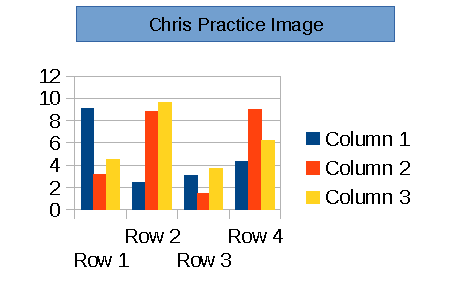
\includegraphics[scale=0.64]{figs/practiceimage}
  \caption{My image for practice. }
  \label{fig:practiceimage}
\end{figure}

This paragraph will show things like
{\em italics} and {\bf bold}.  Also,
I can add comments in two ways.
% Percent starts a comment
50\% of the time you want a slash
in front.  
\MYcomment{If type 
sdsd
dsd
sdsd
ds
dsd
sds}
\MYfigureref{fig:practiceimage} is great!



Sprinting policies have complex effects on
response time.  Seemingly subtle increases or
decreases in budget and timeout can degrade response time.
\MYfigureref{fig:draw-sprintmanager} depicts task
execution under a sprinting policy using a 1-second timeout.
In this example, timeouts trigger sprinting for
tasks 1 and 2, draining the budget.  The remaining tasks must
execute at the sustained processing rate.  Here,
sprinting too aggressively allows queuing delay
to slow down tasks 4, 5 and 6.  However,
increasing the timeout has mixed effects.
Under a 3-second timeout, response time degrades
for the same workload.  This policy is too
conservative and does not exhaust the sprinting
budget.  Under a 2-second timeout, response time
improves by 25\%.  

It is challenging to set good
sprinting policies.  Policies based on human
intuition often consider a small portion of
possible settings and perform poorly when
workloads or hardware change.
In early work, we have started to explore a model-driven approach that sets sprinting policies based on their expected response time. To be precise, we propose a class of performance models that accept the following types of input: arrival rate, sustained processing rate, sprint rate and sprinting budget. Our models characterize response time and sprinting frequency.

A key component of early success with modeling computational sprinting has be the use of random decision forests.  We use this graphical learning method to map marginal sprint rate (i.e the rate for a fully sprinted execution), workload, and sprint policies to effective sprint rate (i.e the rate that amortizes the dynamic runtime factors)--- changing a difficult non-separable problem into distinct solvable parts.  Specifically, the effect sprint rate can be fed into classic queuing models and simulators to predict response time.  


We have already evaluated the accuracy of our approach across five workloads on a dedicated machine using DVFS for sprinting. Figure~\ref{fig:xerror-ycdf-zworkloads} plots relative error for each workload. The curves for all of the workloads are close in shape. Jacobi, Stream, NN, Leukocyte, and BFS had median error below 5\%. Across all workloads, 75$^{th}$ percentile error was below 10\%.
We observed similar results on other architectures. Query execution kernels, whether constrained by compute, memory or synchronization, did not affect our approach's accuracy.  This is because our workload profiler accurately calibrates our approach for each kernel. Leukocyte has strong workload execution phases.  Some phases are more amenable to computational sprinting than others.  Nonetheless, our approach translates between marginal and effective sprint rate actively, using only workload-specific profiles.

\noindent {\bf Related Work:} 
Queuing models can predict response time for server systems~\cite{stewart2013zoolander}.
However, these models assume queuing delay and
service time are independent.  Interdependent queuing and service times lead to complicated and fragile models~\cite{Gardner:Sigmetric15:redundant,morris2016sprint}.
When the focus is throughput, rather than response time, tree based offline profiling techniques work well and nearly optimally~\cite{zhang2016pupil,mishra2017esp,kelley-icac-2015}. If profiles change during online execution, agent-based game theoretic approaches can provide optimal throughput-oriented sprinting policies~\cite{Fan:ASPLOS16:SprintGame,zahedi2017computational}.  {\em Our work targets the very challenging problem of understanding the impact of sprinting on response time.}




\bibliographystyle{abbrv}
\bibliography{bibliography}


\end{document}



